\textbf{Cubie} - An individual cube-shaped element of the puzzle. The Rubik's Cube has 26 cubies (excluding the non-visible cubie at the centre of the cube), and the Kilominx has 20 cubies (sometimes referred to as "\textbf{kubies}" - Kilominx cubies).

\textbf{Face} - A face of the puzzle, which can be twisted to change the state of the puzzle. The Rubik's Cube has 6 faces, while the Kilominx has 12 faces.

\textbf{Twist} - A twist is a rotation of a face of the puzzle. A twist is only valid if the face is aligned with the rest of the puzzle when the twist is completed. Twists are the basic moves that can be made on the puzzle to change its state. The Rubik's Cube has 6 faces, and each face can be twisted in 3 different ways (90 degrees clockwise, 90 degrees counterclockwise, or 180 degrees). The Kilominx has 12 faces, and each face can be twisted in 4 different ways (72 degrees clockwise, 72 degrees counterclockwise, 144 degrees clockwise, or 144 degrees counterclockwise).

\textbf{Move Notation}\label{section:moves} - Twists on the Rubik's Cube can be represented in a shorthand notation \cite{rubiksnotation}, where a letter represents a \textbf{clockwise} twist of the face represented by that letter. If the letter is followed by an apostrophe (e.g. $U'$, read as "U Prime"), it represents a \textbf{counterclockwise} twist of the face. If the letter is followed by the number 2 (e.g. $U2$), it represents \textbf{two clockwise} twists of the face (a 180-degree twist). The letters used to represent the faces of the Rubik's Cube are as follows:
\begin{multicols}{2}
\begin{itemize}
    \item $U$ - Up
    \item $L$ - Left
    \item $B$ - Back
    \item $F$ - Front
    \item $R$ - Right
    \item $D$ - Down
\end{itemize}
\end{multicols}

The notation I defined for the Kilominx is similar, but instead uses up to three letters to represent the faces of the puzzle. In addition, to represent a \textbf{double counterclockwise} twist, the face is followed by a 2 and an apostrophe (e.g. $U2'$). The letters used to represent the faces of the Kilominx are as follows:
\begin{multicols}{2}
\begin{itemize}
    \item $U$ - Up
    \item $L$ - Left
    \item $BL$ - Back Left
    \item $DL$ - Down Left
    \item $DBL$ - Down Back Left
    \item $DB$ - Down Back 
    \item $F$ - Front
    \item $R$ - Right
    \item $BR$ - Back Right
    \item $DR$ - Down Right
    \item $DBR$ - Down Back Right
    \item $D$ - Down
\end{itemize}
\end{multicols}

\textbf{Kilominx Cubie Notation} - In order to make it easier to determine which Kilominx cubie belongs in which position, I defined a notation which names the cubies based on their positions. The cubie notations are shown below in \textbf{\hyperref[fig:kubies]{Figure 2}}.

\begin{figure}[h]
    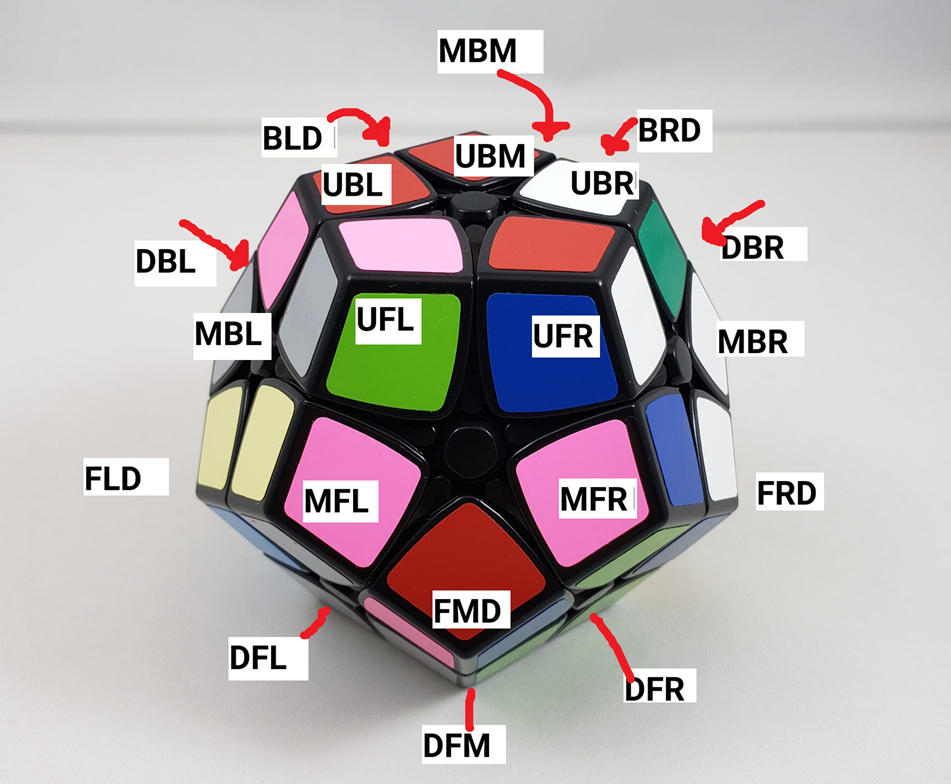
\includegraphics[width=0.8\textwidth]{kilominx_indices_guide}
    \centering
    \caption{An image of a Kilominx, with each cubie labelled based on its position.}
\end{figure}
\label{fig:kubies}